
\section{Aufgaben}

\subsection{Funktion des Codes}

\begin{itemize}
    \item Alle Befehlen müssen funktionieren und den Datenspeicher verändern
    \item Direkte und indirekte Addressierung
    \item Timerfunktion ohne / mit Berücksichtigung der Bits im OPTION-Register (e / o)
    \item Interrupt für Timer 0
    \item Interrupt für INT (RB0)
    \item Interrupt RB4-RB7
    \item ADDWF PCL mit Berücksichtigung von PCLATH (TPicSim101)(theor. Für CALL und GOTO; geprüft an Hand des Codes)
\end{itemize}

\subsection{Funktionen der Gui}
\begin{itemize}
    \item Datenspeicher visualisieren
    \item Den Text der LST datei visualisieren
    \item Die RA und Tris Pins müssen visualisiert werden und per Maus gesetzt werden können
    \item Breakpoints also Debugging mit der Visualisierung der LST dateien
    \item Highlighting des aktuellen (nächsten) Befehls im LST-Fenster 
    \item Spezialregister darstellen
    \item Laufzeit darstellen
    \item Steuerpult mit Start Stop und Step in
\end{itemize}

\begin{figure}[h!]
    \centering
    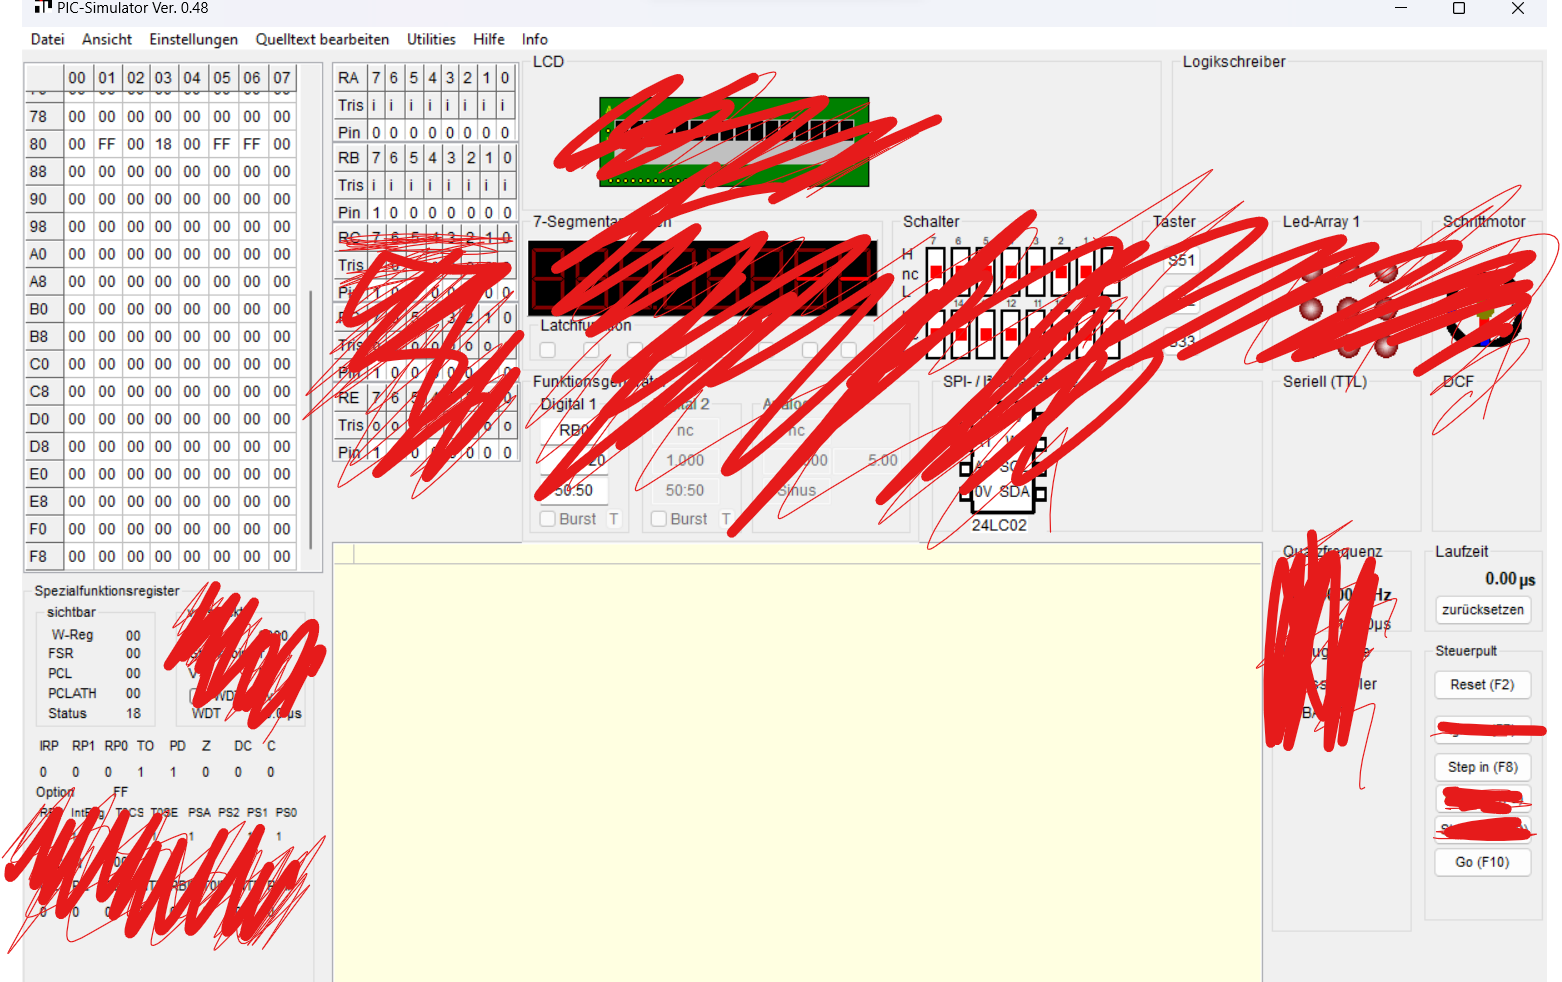
\includegraphics[width=12cm]{input/Screenshot 2023-05-09 111703.png}
    \caption{lehmann-Pic bearbeitet}
    \label{fig:meine-grafik}
\end{figure}

\begin{figure}[h!]
    \centering
    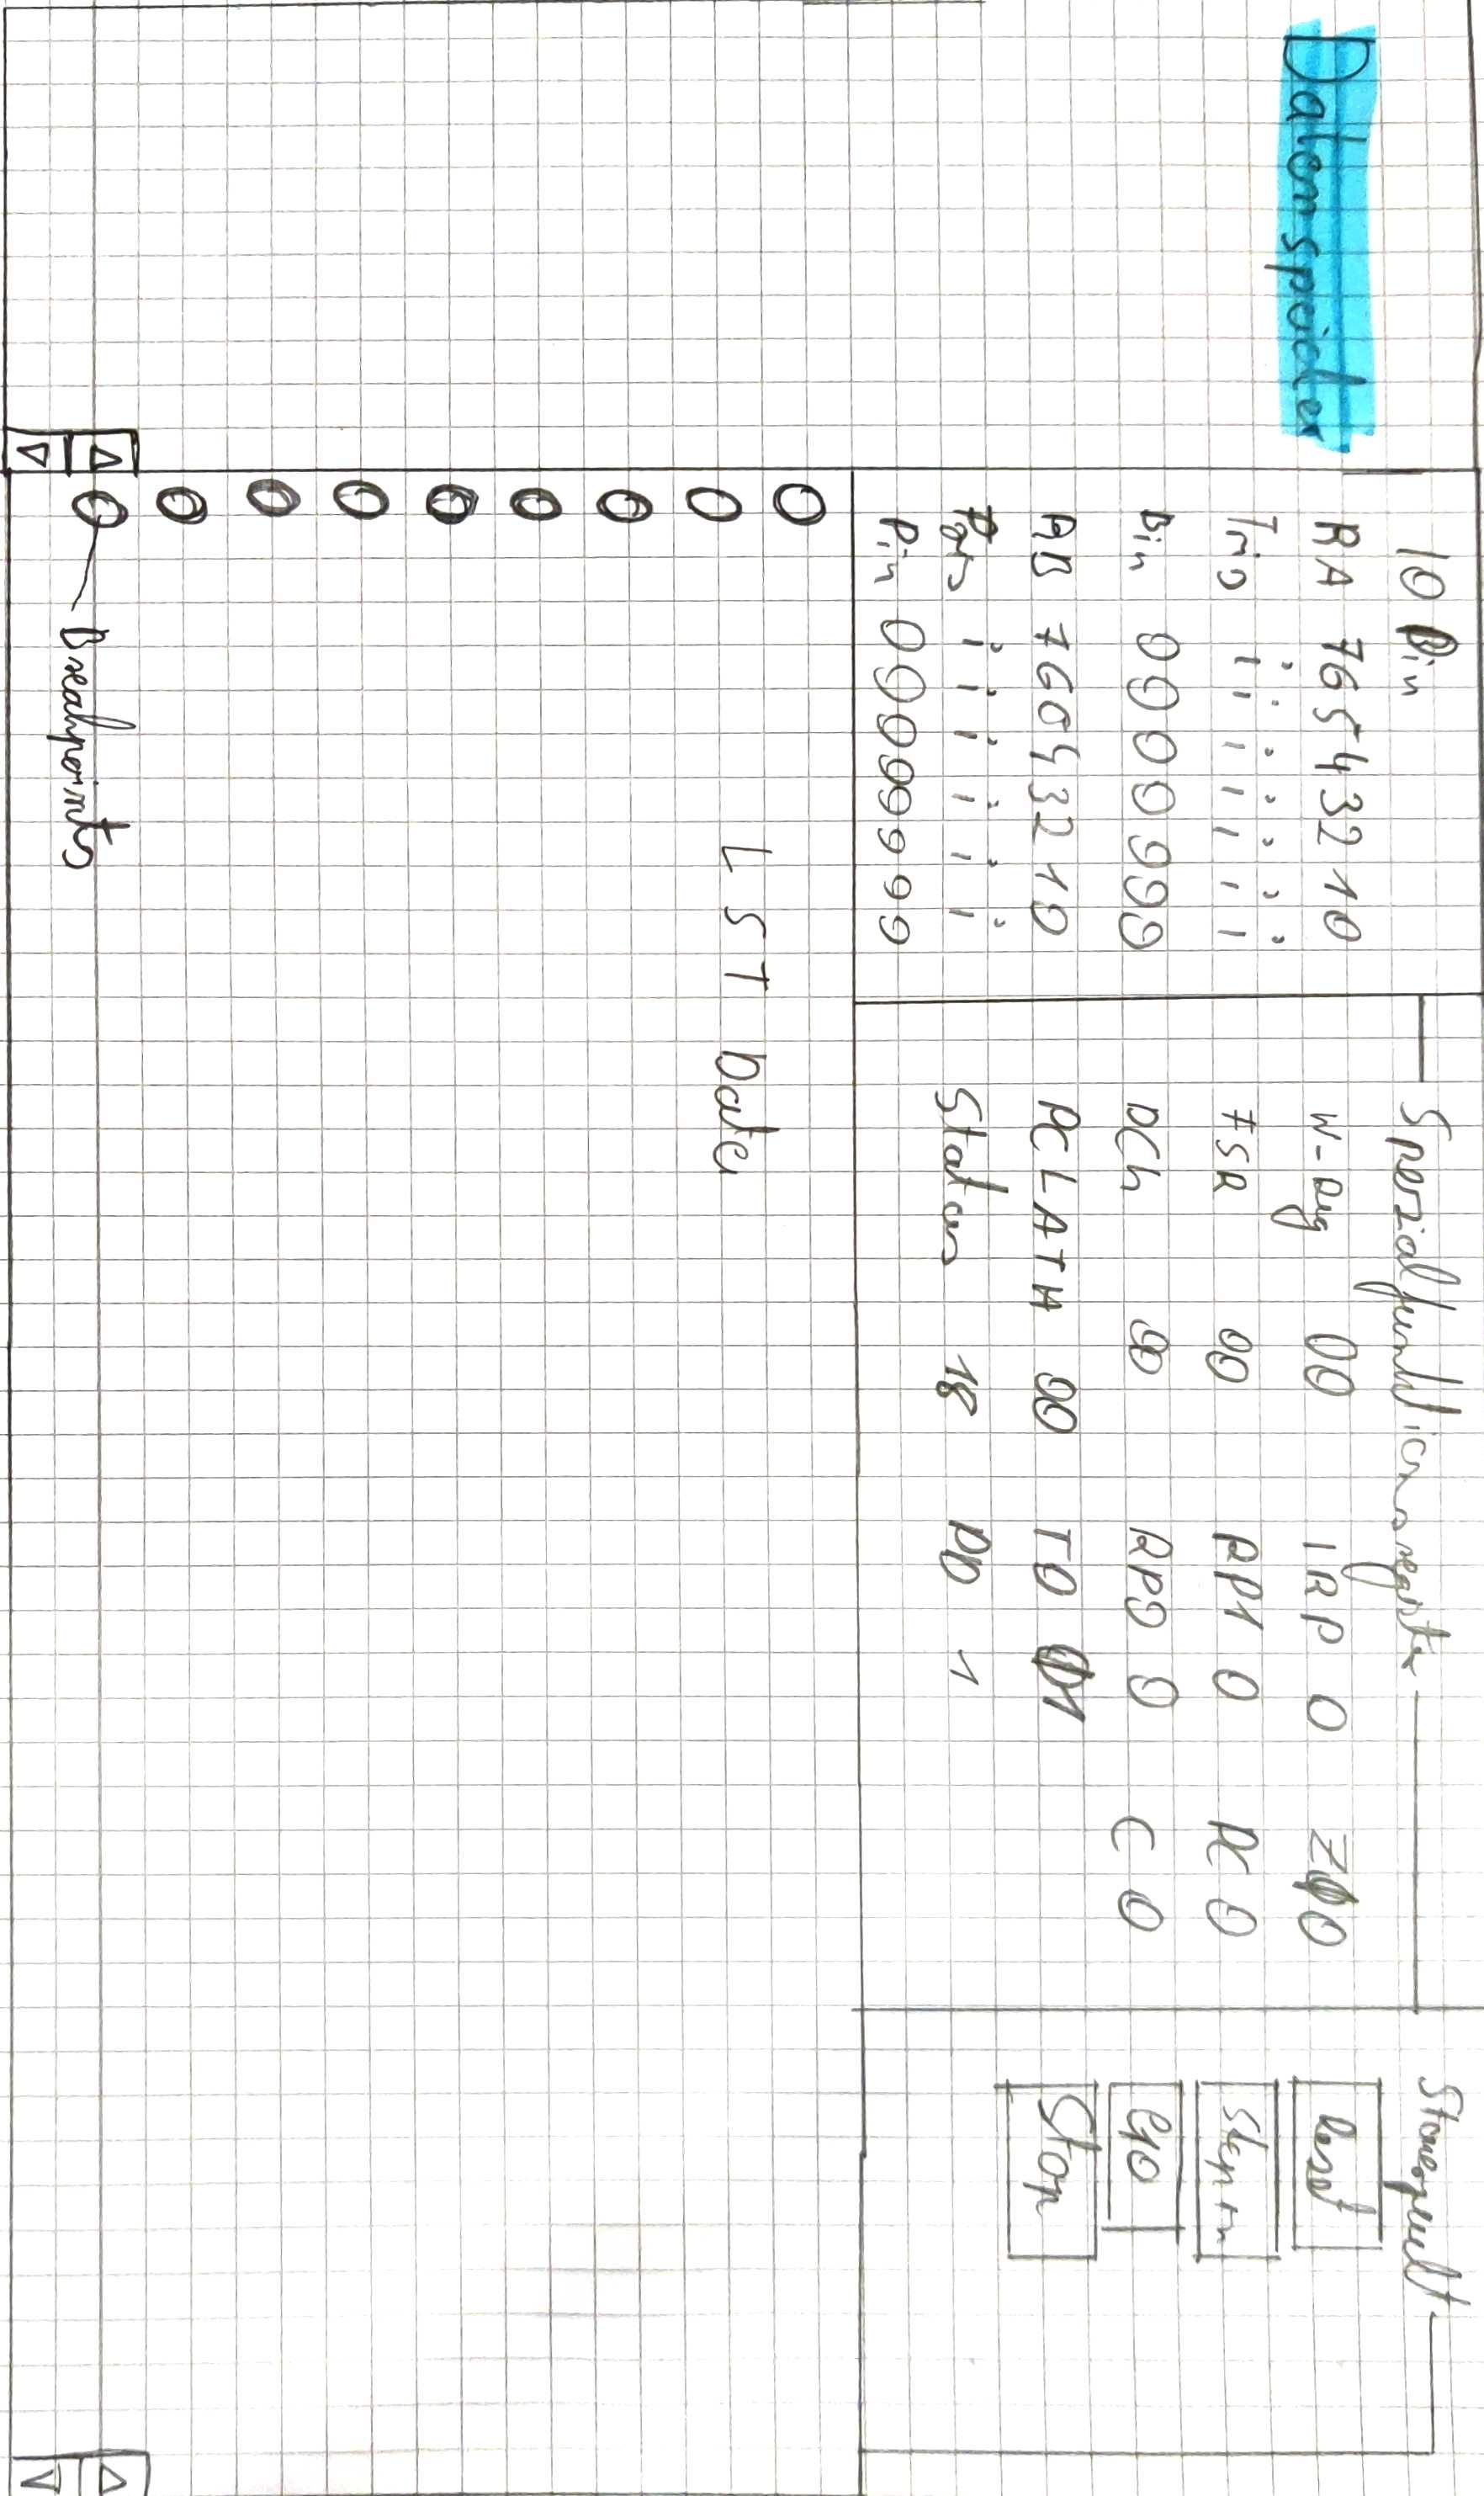
\includegraphics[angle=90,width=12cm]{input/Mock-up-Pic.jpg}
    \caption{Mock-Up-Pic}
    \label{fig:mock-up.pic}
\end{figure}
   
